% generated by src/r2/paper_assets (make_paper_assets.py figures); do not edit by hand
% provenance: fig4_heldout generated by src/r2/paper_assets on 2026-10-15 04:07 from data/r2/tables/
%   heldout_estimators.csv (modified 2026-10-14 20:06): universe = global, eval_subset = all_evaluable, reference in {encode, enets2, pert_pooled}; score in the plotted list
%   heldout_evidence_status.csv (modified 2026-10-14 20:08): reference in {encode, enets2, pert_pooled}
%   obs_heldout_status.csv (modified 2026-10-14 20:37): universe = global, reference = encode, status in {unobserved, observed_neg}: mean_cred_em (EM credibility by evidence status)
%   (constants): LOW_SUPPORT_TFS, LOW_SUPPORT_POS from r2.heldout_eval
\begin{figure}[tbp]
  \centering
  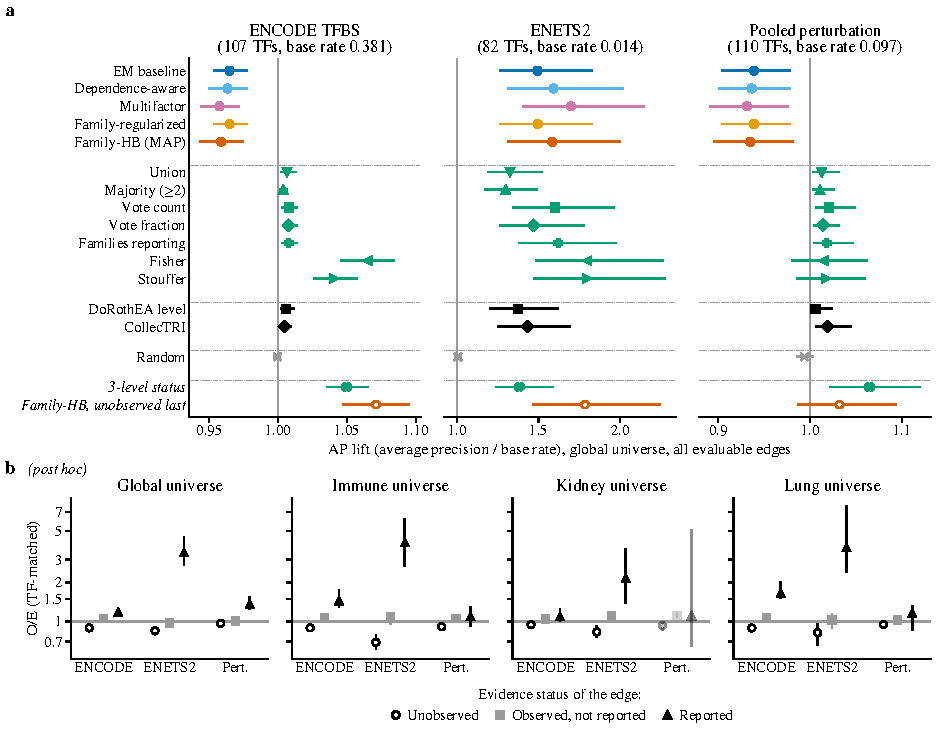
\includegraphics[width=\textwidth]{fig4_heldout.pdf}
  \caption{\textbf{Held-out evaluation in the global universe.} (a) AP lift of every score on all evaluable edges, with 95\% TF-bootstrap intervals; the vertical line marks a random ranking. Open italic rows are post hoc mechanism scores (the 3-level evidence status and Family-HB with unobserved edges ranked last); Family-HB (MAP) is the posterior-mode fit used in the paired tests. Family-HB: ENCODE 0.96 [0.94, 0.98], ENETS2 1.59 [1.31, 2.00], pooled perturbation 0.94 [0.90, 0.98]; Fisher: 1.07 [1.05, 1.08], 1.80 [1.48, 2.27], 1.01 [0.98, 1.06]; EM: 0.96 [0.95, 0.98], 1.49 [1.26, 1.83], 0.94 [0.90, 0.98]. (b) Positives among unobserved, observed but unreported, and reported edges relative to the TF-matched expectation (95\% TF-bootstrap intervals; faded: fewer than 10 TFs with positives or fewer than 20 positives); the whole panel is post hoc. Global universe, unobserved edges: ENCODE 0.89 [0.88, 0.91], ENETS2 0.85 [0.78, 0.90], pooled perturbation 0.97 [0.95, 0.98]; observed negatives 1.05 [1.04, 1.05] (ENCODE). Unobserved edges are depleted of positives in every universe (O/E 0.69 to 0.95 in the tissue universes), whereas the missing-at-random latent-class estimators give them a higher mean credibility than observed negatives (ENCODE-evaluable edges: Family-HB 0.0031 vs 0.00099; EM 0.0068 vs 0.0021): coverage is informative (inference: not missing at random).}
  \label{fig:heldout}
\end{figure}
